\section{Repository Pattern}
Repository pattern blev implementeret ved brug af forskellige dele og lag. I dette afsnit vil de forskellige dele blive beskrevet. 
I starten var tanken med repository-pattern, at alle klasseren i model blev tilknyttet et repository, der indeholdt de gængse CRUD-operationer (Create, Read, Update, Delete) på databasen i forbindelse med hver model. Hvert repository blev nedarvet fra et interface, dette er gjort på baggrund ad DIP, der gør at i forbindelse med test kan repositoriet mockes ud.
Men efter implementering af flere repository blev, det observeret at koden for de forskellige repositories var stort set identisk, hvilket også kan se på en tidligere version af klassediagrammerne på figur \ref{fig:Repository}.
%\begin{figure}[H]
%	\centering
%	\includegraphics
%	[width=165mm]{figures/Repository.PDF}
%	\caption{Oversigt over alle Repository}
%	\label{fig:Repository}
%\end{figure}

Problemet med den identiske kode i de forskellige repository blev løst ved at lave et generelt template-baseret repository (Generisk repository). Det generiske repository indeholder en template baseret implementering af de enkelte CRUD-operationer. Man kan se metoderne og opbygningen af GenericRepository-klassen på figur \ref{fig:GenericRepository}
\begin{figure}[H]
	\centering
	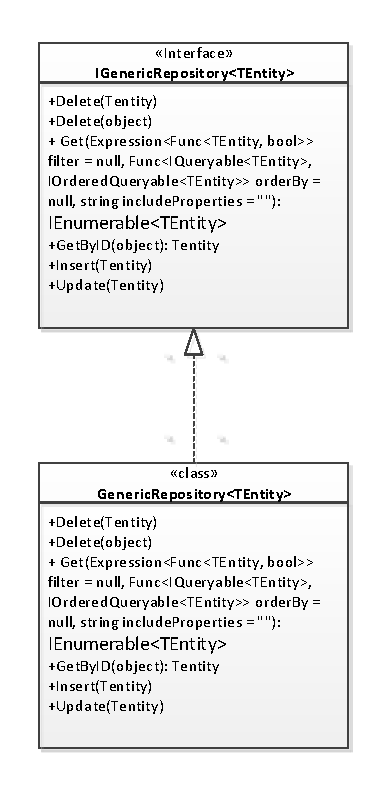
\includegraphics
	[height=180mm]
	{figures/GenericRepository.PDF}
	\caption{GenericRepository opbygning}
	\label{fig:GenericRepository}
\end{figure}


Af særlige interesante metoder i GenericRepository kan nævnet Get-metode, der nok også er den mest anvendte metode i forbindelse med DAL. Denne metode retunere en list af objekter af en given klasse.
Metoden:
\begin{verbatim}
 public virtual IEnumerable<TEntity> Get(Expression<Func<TEntity, bool>> 
 filter = null,Func<IQueryable<TEntity>, 
 IOrderedQueryable<TEntity>> orderBy = null,string includeProperties = "")
\end{verbatim}
Metoden indeholder en række af filtre, ekspression, orders og includeproperties, der gør, at man kan filtre, inkludere og udvælge, hvilke data, der kommer tilbage fra get-metoden. Man kan bl.a. gennem brug af includeproperties komme rundt om EF Lazy-loading. 

GenericRepository's template implementering bliver tilgået igennem unitofwork-klassen. 
UnitOfWork-klassen indeholder de forskellige GenericRepositories, så hvis der skal arbejdes på de forskellige repositories blev de tilgået igennem denne. UnitOfWork-klassen er udarbejdet på den måde, at første gang de et af de genericRepository bliver tilgået oprettes et nyt repository og næste gang dette repository skal tilgås bliver de tidligere opretttet genericRepository retuneret.
UnitOfWork-klassen indeholder desuden også en save-metode og en dispose-metode. Det er disse metoder som comitter til databasen.
UnitOfWork-klassen kan ses på nedenstående klasse diagram på figur \ref{fig:UnitOfWork1}
\begin{figure}[H]
	\centering
	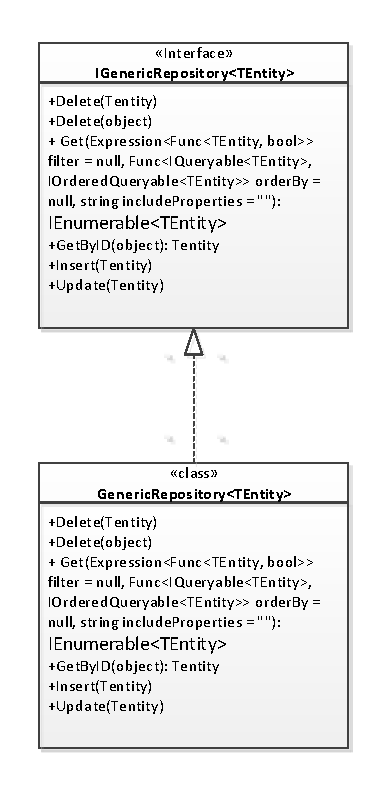
\includegraphics
	[height=180mm]{figures/UnitOfWork1.PDF}
	\caption{UnitOfWork opbygning}
	\label{fig:UnitOfWork1}
\end{figure}

Repository-pattern med unitofWork er som allerede påpeget valgt for at adskille buisness-logikken fra DAL.
